%! Author = Omar Iskandarani
%! Date = 5/4/2025

\section{Afleiding van de tijddilatatieformule binnen VAM}\label{sec:appendix_1}

Binnen het Vortex Æther Model (VAM) ontstaat tijddilatatie niet uit ruimtetijdkromming, maar uit lokale energetische eigenschappen van het ætherveld, zoals rotatie (vorticiteit), drukgradiënten en topologische eigenschappen van wervelstructuren. De lokale klokfrequentie van een wervel—geassocieerd met een elementair deeltje of een macroscopisch object—is afhankelijk van zowel de interne kernrotatie als externe omgevingsinvloeden zoals zwaartekrachtsvelden en frame-dragging.

De tijddilatatiefactor $\frac{d\tau}{dt}$ wordt in VAM uitgedrukt als een samengestelde correctie op de universele tijd $t$, waarin de lokale "eigenklok" $\tau$ trager tikt onder invloed van:

1. Vervorming van ætherstroom rond een wervelkern;
2. Externe gravitationele vorticiteit veroorzaakt door massa;
3. Roterende achtergrondvelden.

We leiden de volgende formule af:

\begin{equation}
\frac{d\tau}{dt} = \sqrt{1 - \frac{C_e^2}{c^2} e^{-r/r_c} - \frac{2G_\text{swirl} M_\text{eff}(r)}{r c^2} - \beta \Omega^2}
\end{equation}

Elke term vertegenwoordigt een fysisch mechanisme:

\begin{itemize}
  \item \textbf{Term 1: Kernrotatie (lokale swirl)}
  \[
  \frac{C_e^2}{c^2} e^{-r/r_c}
  \]
  Deze term is afgeleid uit de intrinsieke hoeksnelheid $\Omega_\text{core}$ van de wervelkern. De tangentiële snelheid $C_e$ is de maximale swirl op de kernrand, en $r_c$ is de straal van de wervelkern. De exponentiële factor $e^{-r/r_c}$ geeft de afname van invloed weer op afstand $r$ buiten de kern. Deze term representeert de tijdvertraging als gevolg van lokale ætherrotatie.

  \item \textbf{Term 2: Zwaartekrachtsveld (vorticiteit-geïnduceerde potentiaal)}
  \[
  \frac{2 G_\text{swirl} M_\text{eff}(r)}{r c^2}
  \]
  Deze term bootst de klassieke gravitationele roodverschuiving na, maar met een alternatieve zwaartekrachtsconstante $G_\text{swirl}$ die volgt uit ætherparameters zoals dichtheid en swirlkracht. De effectieve massa $M_\text{eff}(r)$ kan hier worden opgevat als de æther-vortexenergie binnen straal $r$, i.p.v. conventionele massa. Deze term komt voort uit het drukdeficit door externe swirl en vervangt Newtonse zwaartekracht.

  \item \textbf{Term 3: Macroscopische rotatie (frame-dragging)}
  \[
  \beta \Omega^2
  \]
  Deze term representeert frame-dragging-effecten binnen een draaiende wervelconfiguratie (vergelijkbaar met het Kerr-metriek-effect in GR). De factor $\Omega$ is de rotatiesnelheid van het macroscopisch object (bijv. planeet of neutronenster), en $\beta$ is een koppelingsconstante die afhangt van ætherparameters. Deze term veroorzaakt extra vertraging van lokale tijd door circulatie van het omringende ætherveld.

\end{itemize}

\begin{figure}[H]
  \centering
  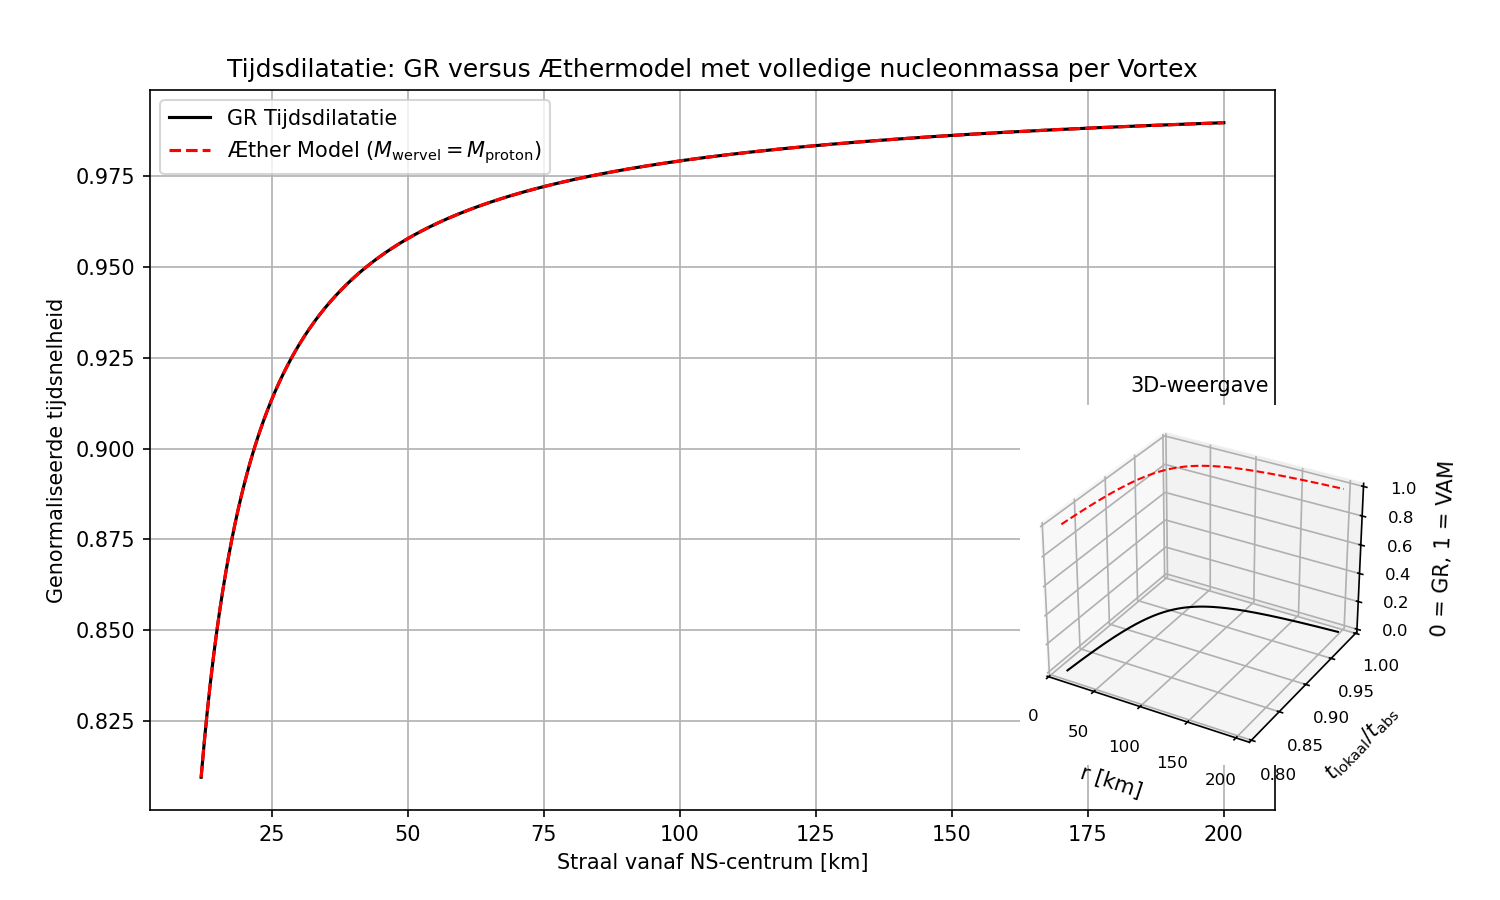
\includegraphics[width=0.85\textwidth]{07-TimeDilationGRVsVAM_nl}
  \caption{
  \textbf{Vergelijking van tijddilatiemodellen:} De tijddilatatieformule uit de Algemene Relativiteitstheorie (GR) \(\sqrt{1 - 2GM/(rc^2)}\) wordt vergeleken met de VAM-formule afgeleid in Eq. (A1), die lokale afname van wervelhoeksnelheid, vorticiteit-geïnduceerde zwaartekrachteffecten en rotatie-geïnduceerde frame-dragging omvat. De krommen lopen uiteen naarmate lokale rotatie dominant wordt, wat verschillen benadrukt in hoge-dichtheidsregimes of wervelgebaseerde systemen.
  }
  \label{fig:GRvsVAMTimeDilation}
\end{figure}

De bovenstaande vergelijking is analoog aan relativistische formules, maar wortelt in vloeistofmechanische oorsprong. Experimenteel kunnen componenten van deze formule worden teruggevonden in tijddilatatie van GPS-klokken (zwaartekracht), Lense-Thirring-effecten (rotatie), en hypothetische laboratoriummetingen van kernrotaties op quantum- of wervelschaal.